
\section{ Распределения }
На рисунках 1-6 представлены графики для различных хэш функций:

\noindent\begin{minipage}[h!]{0.45\linewidth}
    \begin{center}
        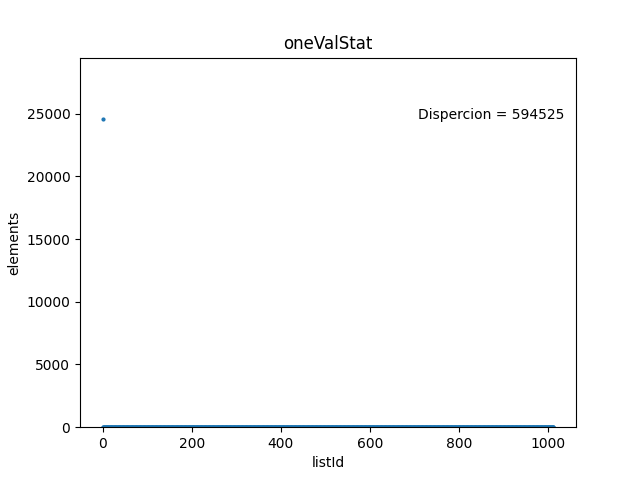
\includegraphics[width = 1\linewidth]{oneValStat.png} \\
        \textit{Рис. 1. хэш функция одного значения }
    \end{center} 
\end{minipage}
\begin{minipage}[h!]{0.45\linewidth}
    \begin{center}
        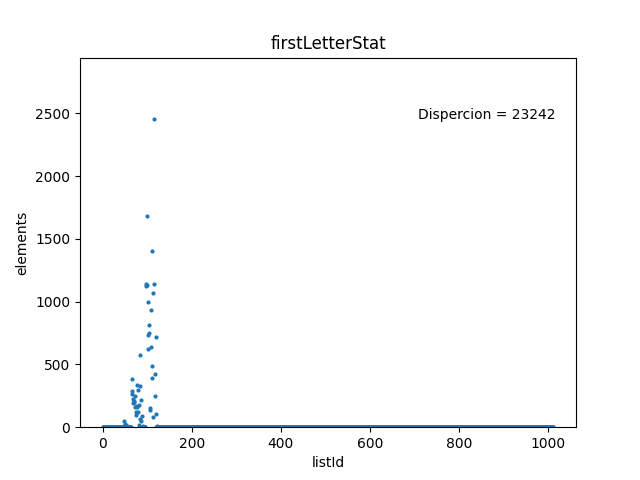
\includegraphics[width = 1\linewidth]{firstLetterStat.png} \\
        \textit{Рис. 2. хэш функция первой буквы }
    \end{center} 
\end{minipage}

\noindent\begin{minipage}[h!]{0.45\linewidth}
    \begin{center}
        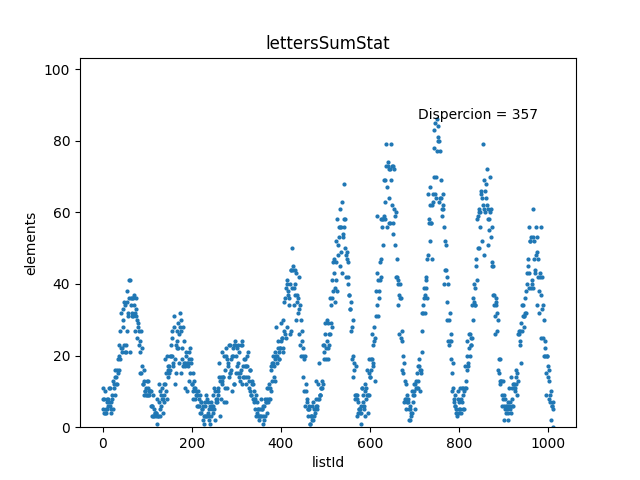
\includegraphics[width = 1\linewidth]{lettersSumStat.png} \\
        \textit{Рис. 3. хэш функция суммы букв }
    \end{center} 
\end{minipage}
\begin{minipage}[h!]{0.45\linewidth}
    \begin{center}
        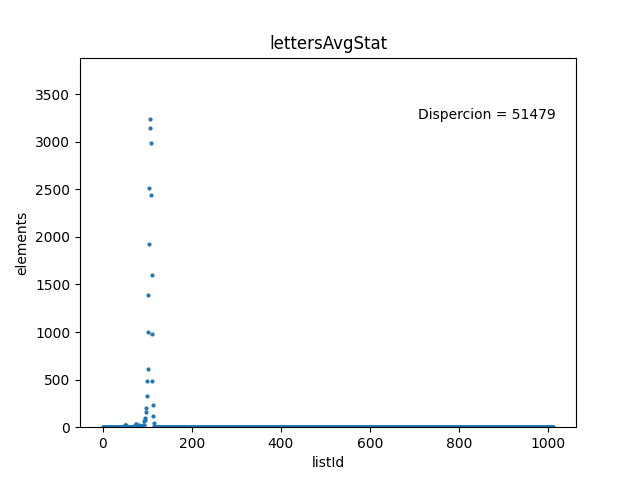
\includegraphics[width = 1\linewidth]{lettersAvgStat.png} \\
        \textit{Рис. 4. хэш функция среднего значения\\ кодов символов }
    \end{center} 
\end{minipage}

\noindent\begin{minipage}[h!]{0.45\linewidth}
    \begin{center}
        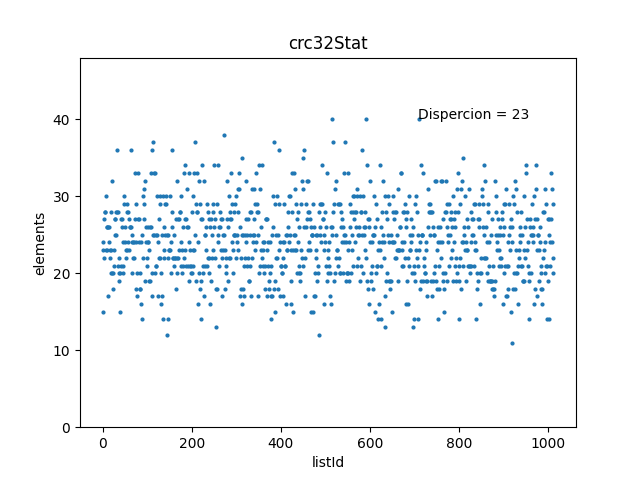
\includegraphics[width = 1\linewidth]{crc32Stat.png} \\
        \textit{Рис. 5. crc32 }
    \end{center} 
\end{minipage}
\noindent\begin{minipage}[h!]{0.45\linewidth}
    \begin{center}
        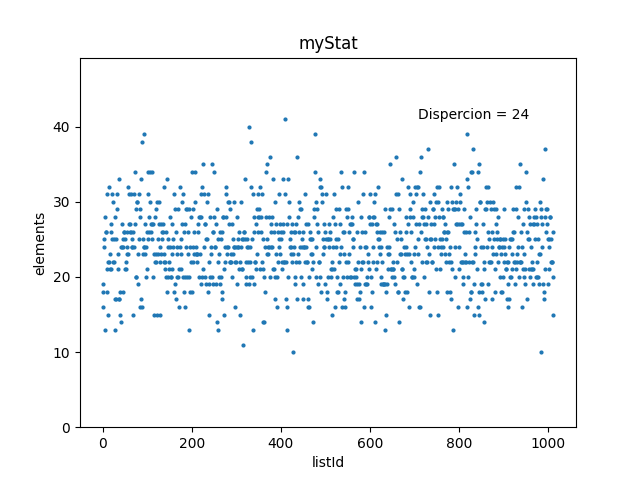
\includegraphics[width = 1\linewidth]{myStat.png} \\
        \textit{Рис. 6. моя хэш функция из 1 семестра }
    \end{center} 
\end{minipage}

\newpage

\section{ Вывод }

Хочется отметить, что моя хэш функция из 1 семестра работает на равне с crc32 (по распределению). \\ [0.1cm]
Видно, что лучше всего себя показывает crc32. Его я и буду использовать для следующей лабараторной работы.